\documentclass[a4paper, 12pt, twoside]{article}
\usepackage[left = 3cm, right = 3cm]{geometry}
\usepackage[english]{babel}
\usepackage[utf8]{inputenc}
\usepackage{mathtools}
\usepackage{amssymb}
\usepackage{amsmath}
\usepackage{multicol}
\usepackage{tikz}
\usetikzlibrary{positioning}

\begin{document}

\title{Understanding Root Spaces and Eigenspaces}
\date{}
\author{\textit{by Tyler Wright}}
\maketitle

\section{Preface}

We will be considering $f, \text{id}$ in $\mathcal{L}(V, V)$, where $V$ is a 
vector space over the field $K$ and id is the identity function on $\mathcal{L}(V, V)$.

\section{The Root Space}

The root space for some $\lambda$ in $K$ is $V(\lambda) \subseteq V$ where for all 
$v$ in $V(\lambda)$: \begin{gather*}
    (f - \lambda\text{id})^r(v) = 0_{V},
\end{gather*} for some $r$ in $\mathbb{Z}_{> 0}$ called the height of $v$, denoted by $h(v)$.
Note that the height of vectors in the root space may vary and: \begin{itemize}
    \item $V(\lambda) \neq \{0\}$ if and only if $\lambda$ is an eigenvalue,
    \item $V(\lambda)$ is $f$-invariant,
    \item The intersection of two root spaces is not $\{0\}$ if and only if
    they are over the same value.
\end{itemize}

\section{The Eigenspace}

The eigenspace for some $\lambda$ in $K$ is $E(\lambda) \subseteq V(\lambda) \subseteq V$
where for all $v$ in $E(\lambda)$: \begin{gather*}
    (f - \lambda\text{id})(v) = 0_{V}.
\end{gather*}

\newpage

\section{Mapping from the Root Space to the Eigenspace}

For a given (non-zero) root space $V(\lambda)$, for each $v$ in $V(\lambda)$,
suppose we apply $(f - \lambda\text{id})$ to it $h(v) - 1$ times, take
$w = (f - \lambda\text{id})^{h(v) - 1}(v)$. As $(f - \lambda\text{id})^{h(v)}(v) = 0$ by
definition, $(f - \lambda\text{id})(w) = 0$, thus $w$ is an eigenvalue.
\\[\baselineskip]
We can visualise this with a graph (of stacks) where the directed edges represent applications
of $(f - \lambda\text{id})$: \begin{center}
    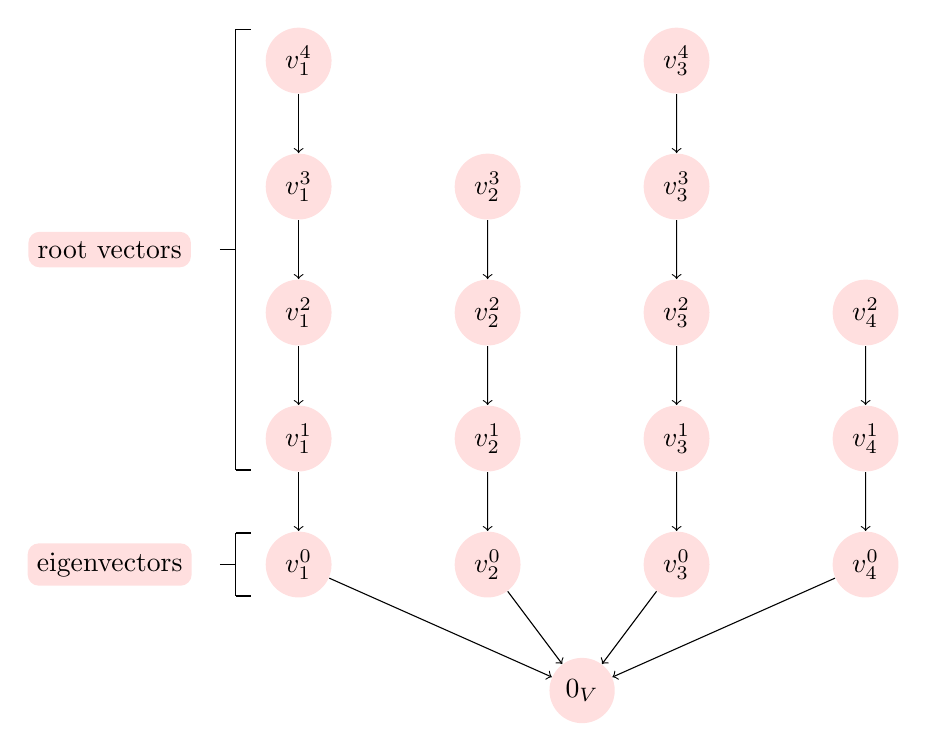
\begin{tikzpicture}
        [scale=.8,auto=left,every node/.style={circle,fill=pink!50}]
        \node (a5) at (0, 8) {$v_1^4$};
        \node (a4) at (0, 6) {$v_1^3$};
        \node (a3) at (0, 4) {$v_1^2$};
        \node (a2) at (0, 2) {$v_1^1$};
        \node (a1) at (0, 0) {$v_1^0$};

        \node (b4) at (3, 6) {$v_2^3$};
        \node (b3) at (3, 4) {$v_2^2$};
        \node (b2) at (3, 2) {$v_2^1$};
        \node (b1) at (3, 0) {$v_2^0$};

        \node (c5) at (6, 8) {$v_3^4$};
        \node (c4) at (6, 6) {$v_3^3$};
        \node (c3) at (6, 4) {$v_3^2$};
        \node (c2) at (6, 2) {$v_3^1$};
        \node (c1) at (6, 0) {$v_3^0$};

        \node (d3) at (9, 4) {$v_4^2$};
        \node (d2) at (9, 2) {$v_4^1$};
        \node (d1) at (9, 0) {$v_4^0$};
        
        \node (zero) at (4.5, -2) {$0_V$};

        \node[rectangle, rounded corners] (e1) at (-3, 5) {root vectors};
        \draw (-1.25,5) -- (-1,5);
        \draw (-1,8.5) -- (-1,1.5);
        \draw (-1,8.5) -- (-0.75,8.5);
        \draw (-1,1.5) -- (-0.75,1.5);

        \node[rectangle, rounded corners] (e2) at (-3, 0) {eigenvectors};
        \draw (-1.25,0) -- (-1,0);
        \draw (-1,0.5) -- (-1,-0.5);
        \draw (-1,0.5) -- (-0.75,0.5);
        \draw (-1,-0.5) -- (-0.75,-0.5);

        \foreach \from/\to in {a5/a4, a4/a3, a3/a2, a2/a1, 
        b4/b3, b3/b2, b2/b1,
        c5/c4, c4/c3, c3/c2, c2/c1, d3/d2, d2/d1, d1/zero, c1/zero, b1/zero, a1/zero}
            \draw[->] (\from) -- (\to);

      \end{tikzpicture}
\end{center} Note that multiple eigenvectors can belong to the same eigenspace.

\section{Eigenvalue Multiplicity}

We have the height of a stack is the multiplicity of the eigenvalue of the stack 
in the \textbf{minimal polynomial}. Thus, for maps with dim$(V)$ distinct eigenvalues,
for each eigenvalue $\lambda$, $V(\lambda) = E(\lambda)$.

\newpage

\section{An Example}

Take the following matrix: \begin{gather*}
    A = \begin{pmatrix}
        2 & 0 & 0 \\
        0 & 2 & 0 \\
        0 & 0 & 2
    \end{pmatrix}.
\end{gather*} We clearly have: \begin{align*}
    p_A(x) &= (x - 2)^3 \\
    m_A(x) &= (x - 2),
\end{align*} demonstrating we have one eigenvalue, 2, with multiplicity 3 in the
characteristic polynomial and multiplicity 1 in the minimal polynomial. We have
a basis $\mathcal{B}_A$ for $E(2)$ where $\mathcal{B}_A = \{e_1, e_2, e_3\},$ 
with a stack representation: \begin{center}
    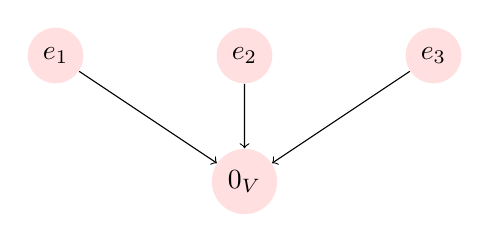
\begin{tikzpicture}
        [scale=.8,auto=left,every node/.style={circle,fill=pink!50}]
        \node (a3) at (0, 0) {$e_1$};
        \node (a2) at (3, 0) {$e_2$};
        \node (a1) at (6, 0) {$e_3$};
        \node (zero) at (3, -2) {$0_V$};

        \foreach \from/\to in {a1/zero, a2/zero, a3/zero}
            \draw[->] (\from) -- (\to);

      \end{tikzpicture}
\end{center} Now consider: \begin{gather*}
    B = \begin{pmatrix}
        2 & 1 & 0 \\
        0 & 2 & 0 \\
        0 & 0 & 2
    \end{pmatrix}, \qquad
    C = \begin{pmatrix}
        2 & 1 & 0 \\
        0 & 2 & 1 \\
        0 & 0 & 2
    \end{pmatrix}.
\end{gather*} It can be seen that $B$ and $C$ both have a single eigenvalue each, being $2$.
However, for example, $e_2$ is not in $E(2)$ of $B$ or $C$. We will consider $B$, we have that:
\begin{align*}
    p_B(x) &= (x - 2)^3 \\
    m_B(x) &= (x - 2)^2,
\end{align*} here the multiplicity of $2$ in the minimal polynomial is $2$ indicating
that there is a stack of height $2$. We have a basis $\mathcal{B}_B$ for $E(2)$ on $B$
where $\mathcal{B}_B = \{e_1, e_3\}$ with a stack representation: \begin{center}
    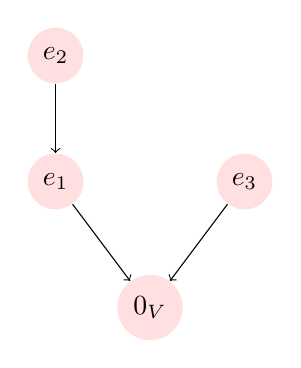
\begin{tikzpicture}
        [scale=.8,auto=left,every node/.style={circle,fill=pink!50}]
        \node (a3) at (0, 0) {$e_1$};
        \node (a2) at (3, 0) {$e_3$};
        \node (a1) at (0, 2) {$e_2$};
        \node (zero) at (1.5, -2) {$0_V$};

        \foreach \from/\to in {a1/a3, a2/zero, a3/zero}
            \draw[->] (\from) -- (\to);

      \end{tikzpicture}
\end{center} Now, for $C$, \begin{align*}
    p_C(x) &= (x - 2)^3 \\
    m_C(x) &= (x - 2)^3,
\end{align*} here the multiplicity of $2$ in the minimal polynomial is $3$ indicating
that there is a stack of height $3$. We have a basis $\mathcal{B}_C$ for $E(2)$ on $C$
where $\mathcal{B}_C = \{e_1\}$ with a stack representation: \begin{center}
    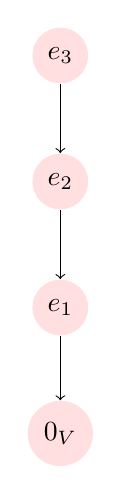
\begin{tikzpicture}
        [scale=.8,auto=left,every node/.style={circle,fill=pink!50}]
        \node (a2) at (0, 4) {$e_3$};
        \node (a3) at (0, 0) {$e_1$};
        \node (a1) at (0, 2) {$e_2$};
        \node (zero) at (0, -2) {$0_V$};

        \foreach \from/\to in {a1/a3, a2/a1, a3/zero}
            \draw[->] (\from) -- (\to);

      \end{tikzpicture}
\end{center}

\end{document}
